% -------------------------------------------------
%  Cache-Optimized, Parallel BA – ICRA 2026 Paper
% -------------------------------------------------
\documentclass[conference]{IEEEtran}

% ---------- Packages ----------
\usepackage{graphicx}
\usepackage{amsmath,amssymb}
\usepackage{booktabs}      % professional tables
\usepackage{siunitx}       % \SI{10}{\micro\second}
\usepackage{subcaption}    % subfigures
\usepackage{hyperref}
\usepackage{amssymb}    % for \checkmark
\usepackage{pifont}     % for more dingbats, if you prefer
\usepackage{listings}      % for code listings
\usepackage{algorithm}     % for algorithms
\usepackage{algpseudocode} % for algorithmic pseudocode
\usepackage{xcolor}        % for colors
\usepackage{enumitem}      % for customizing lists
\newcommand{\cmark}{\checkmark}
\newcommand{\xmark}{\ding{55}}  % or \ensuremath{\times}


% ---------- Bibliography ----------
\bibliographystyle{IEEEtran}
\addtolength{\textfloatsep}{-0.5\baselineskip} % tighter floats

% ---------- Title ----------
\title{Accelerated Bundle Adjustment for Multicore Platforms}

\author{
  \IEEEauthorblockN{First Author\IEEEauthorrefmark{1},
                    Second Author\IEEEauthorrefmark{2}, and
                    Third Author\IEEEauthorrefmark{1}}
  \IEEEauthorblockA{\IEEEauthorrefmark{1}Department of Electronic and Telecommunication Engineering,\\
                    University of Moratuwa, Sri Lanka\\
                    Email: \{first,third\}@uom.lk}
  \IEEEauthorblockA{\IEEEauthorrefmark{2}School of Computer Science and Engineering, NTU Singapore\\
                    Email: second@ntu.edu.sg}
}

\begin{document}
\maketitle
\begin{abstract}
  ***Change This***We present a cache-optimized, highly parallel formulation of classical Bundle Adjustment (BA) that reorganises sparse Jacobians into large dense blocks, exposing the arithmetic to vendor-optimised BLAS APIs. The method scales across embedded multicore CPUs with OpenMP and remains backend-agnostic – it runs unmodified on OpenBLAS, MKL and ARMPL. On a quad-core Cortex-A55 we obtain a \SI{2}{\times} speed-up over Ceres‐Sparse while preserving accuracy on BAL dataset.
\end{abstract}

\begin{IEEEkeywords}
  Bundle Adjustment, BLAS, Parallel Computing, Cache Optimization, Embedded SLAM.
\end{IEEEkeywords}

% ---------- Main Sections ----------
\section{Introduction}\label{sec:intro}


\begin{figure}[t]
  \centering
  
\includegraphics[width=0.9\linewidth]{figs/placeholder}
  \caption{System pipeline overview (placeholder).}
  \label{fig:intro_pipeline}
\end{figure}

\IEEEPARstart{V}{isual} simultaneous localisation and mapping (SLAM) and structure‑from‑motion (SfM) systems 
reconstruct camera motion and 3‑D structure from image sequences and have become indispensable in robotics, 
mixed‑reality, and autonomous navigation~\cite{cadena2016past,hartley2003multiple}.
Modern pipelines split into a front‑end for visual odometry and loop detection and a back‑end for optimisation, typically 
bundle adjustment (BA)\cite{campos2021orb}.
The front‑end is no longer the primary time sink: ORB extractors running on SIMD\cite{rublee2011orb}, FPGA‑accelerated 
ORB variants that reach $>$1.2,kFPS at \SI{2.1}{\watt}\cite{wang2022fpga_orb}, and compact CNN keypoint‑descriptor heads such 
as MobileSP that achieve \SI{4}{ms} inference on a Jetson Xavier NX\cite{zhang2022mobilesp} deliver 
realtime feature tracks even on edge devices.
As a result, the computational bottleneck has migrated to the BA back‑end, which jointly refines camera poses and landmarks 
via nonlinear least‑squares.

On embedded CPUs—from quad‑core Cortex‑A53 to octa‑core automotive SoCs—profiling studies report that BA consumes 
\SIrange{55}{70}{\percent} of the total SLAM runtime despite sliding windows of only 10–15 keyframes~\cite{matthee2024predicting}.
The culprit is not arithmetic intensity but memory behaviour: pointer‑rich sparse data layouts in \textsc{g2o} or \textsc{Ceres} 
trigger cache misses that stall the pipeline for more than 70 \% of cycles~\cite{triggs1999bundle}.

















Several acceleration strategies have been explored to address this bottleneck. 
\textbf{GPUs.}\;PBA~\cite{wu2011multicore} and MegBA~\cite{ren2022megba} deliver over 500~MFLOPS/W on desktop GPUs, 
yet still exceed the power budget of mobile robots.

\textbf{Dedicated hardware.}\;FPGA/ASIC accelerators such as $\pi$‑BA~\cite{qin2019pi} and BAX~\cite{sun2020bax} 
achieve \emph{low‑millisecond} Schur‑complement builds, but only after inserting sizeable on‑chip RAM buffers that 
tame BA's irregular access pattern, inflating LUT/FF counts and power. $\pi$‑BA accelerates just the Schur stage and 
consumes 141.5 Block RAMs—about 98~\% of the 144 BRAMs available on a Kria KR260—leaving little headroom for the 
remainder of a SLAM stack. BAX lowers BRAM pressure with their DAE architecture but had to cap the optimisation window 
to 16 camera poses and 256 landmarks, a setting adequate for synthetic demos yet too restrictive for real deployments, 
and still relies on handcrafted memory banking.

\textbf{Multicore CPUs.}\;State‑of‑the‑art BA solvers such as \textsc{g2o}~\cite{kummerle2011g} and 
\textsc{Ceres}~\cite{agarwal2012ceres} store the Jacobian/Hessian in compressed sparse row/column (CSR/CSC) form and 
drive the solve with sparse‑BLAS plus OpenMP threads. This fits cache‑rich desktop CPUs, but on embedded cores the 
pointer chasing in CSR converts each FLOP into multiple uncached reads, throttling throughput and wasting energy. 
Because CSR indirection keeps arithmetic scattered behind pointer walks, off‑the‑shelf solvers expose no clear compute 
kernel to offload; duplicating the row‑pointer chase would demand on‑chip buffers that mid‑tier FPGAs or NPUs simply lack.

These observations motivate a rethink: Can we keep the light‑weight control flow on the CPU yet off‑load the numerically 
intensive kernels to any attached accelerator—GPU, NPU, or FPGA—through platform‑agnostic interfaces (such as BLAS\cite{BLAS} APIs) and thereby harvest 
substantial speed‑ups?

We present a BA solver designed from scratch for multicore embedded CPUs that turns sparse BA into 
batched dense GEMMs through three principles: (1) \emph{pointer‑free storage} that guarantees stride‑1 access, (2) a 
\emph{tiled two‑phase Schur complement} (T$^{2}$SC) that overlaps memory copies with BLAS, and (3) a 
\emph{BLAS‑centric kernel map} that lets us swap OpenBLAS, MKL, or ARMPL at link time.

Our main contributions are:
\begin{itemize}[leftmargin=*]\setlength\itemsep{2pt}
\item A dense local-ID scheme and landmark-first edge bucketing that eliminate pointer chasing (\S\ref{subsec:parameter_ordering});
\item Flat connectivity arrays enabling $\mathcal{O}(1)$ block lookup across Jacobian, Hessian and Schur 
structures (\S\ref{subsec:connectivity_storage});
\item \textbf{T$^{2}$SC}: a producer--consumer tiled Schur pipeline that hides memory latency behind batched 
GEMM (\S\ref{subsec:t2sc});
\item A complete mapping of BA kernels to Level-3 BLAS, allowing drop-in use of vendor libraries (\S\ref{subsec:blas_apis});
\item An open-source C++ implementation that matches \textsc{g2o}'s final $\chi^{2}$ on the BAL benchmark while reducing 
the 10-iteration wall-time by up to $3\times$ (Core~i9-9900K) and $2\times$ (Cortex-A53) (\S\ref{sec:results}).
\end{itemize}

% \subsection*{E. Paper Organisation}
% Section II surveys related work; Section III gives a high‑level overview; Section IV details the methodology; Section V 
% outlines the experimental protocol; Section VI discusses results and ablations; Section VII concludes and sketches future 
% directions.
% %--------------------------------------------------------------

% \begin{table}[b]
%   \caption{Summary of contributions (placeholder)}
%   \label{tab:intro_contrib}
%   \centering
%   \begin{tabular}{@{}ll@{}}
%     \toprule
%     Problem & Our Remedy \\ \midrule
%     Sparse cache misses & Dense block reorder \\
%     Serial solver & OpenMP parallel BA \\ \bottomrule
%   \end{tabular}
% \end{table}

%%%%%%%%%%%%%%%%%%%%%%%%%%%%%%%%%%%%%%%%%%%%%%%%%%%%%%%%%%%%%%%%%%%%%%%%%%%%%%
% Background & Related Work
%%%%%%%%%%%%%%%%%%%%%%%%%%%%%%%%%%%%%%%%%%%%%%%%%%%%%%%%%%%%%%%%%%%%%%%%%%%%%%
\section{Background \& Related Work}
\label{sec:related}

This section surveys the landscape that motivates our cache-optimized, BLAS-centric
approach.  We group prior art into five themes: the role of bundle adjustment (BA)
in SLAM and structure-from-motion (SfM), numerical strategies based on
Levenberg–Marquardt (LM) and the Schur complement, widely-used BA software
libraries, dense BLAS–oriented acceleration, and finally embedded or
multicore‐specific implementations.

%------------------------------------------------------------------------
\subsection{Bundle Adjustment in SLAM and SfM}
\label{sec:ba_slam}

BA refines camera poses $\mathbf{T}_{wc}$ and 3-D points
$\mathbf{X}\!\in\!\mathbb R^{3}$ by minimizing the reprojection cost
$\sum_{i,j}\!\rho\!\bigl(\|\mathbf r_{ij}\|^{2}\bigr)$, where
$\mathbf r_{ij}$ is the pixel error of landmark~$j$ in image~$i$ and
$\rho(\cdot)$ is a robust loss~\cite{Hartley2003,Lourakis2009}.
%
\textbf{Global} pipelines such as COLMAP perform full BA after incremental
reconstruction~\cite{Schonberger2016}, whereas real-time SLAM systems
(e.g.\ ORB-SLAM3~\cite{MurArtal2021}) use \textbf{local} sliding-window BA to
bound latency.  Window size, marginalization policy, and graph sparsity
(edge fixing vs.\ landmark elimination) directly impact accuracy and runtime;
comparative studies are given in~\cite{Engel2018,Usenko2019,Pfrommer2020}.

%------------------------------------------------------------------------
\subsection{Levenberg--Marquardt and the Schur Complement}
\label{sec:lm_schur}

LM blends Gauss–Newton with a trust-region damping term
$\lambda\operatorname{diag}(\mathbf J^{\!\top}\mathbf J)$, yielding robust
convergence for ill-conditioned BA~\cite{Lourakis2005}.  Eliminating
landmarks via the two-phase Schur complement reduces the normal equations to
a camera-only system
$\mathbf S\Delta\boldsymbol\theta=-\mathbf g$ whose assembly and solution
dominate the computational cost~\cite{Agarwal2012,Chen2022}.  Recent work
explores block-Jacobian tiling~\cite{Merry2016} and hierarchical damping
schemes~\cite{Zhang2023}, yet memory traffic for forming $\mathbf S$
remains the primary bottleneck.

%------------------------------------------------------------------------
\subsection{General-Purpose BA Libraries}
\label{sec:ba_libs}

\textbf{g2o}~\cite{Kuemmerle2011}, \textbf{Ceres}~\cite{Agarwal2012} and
\textbf{SBA}~\cite{Ni2007} expose flexible graph abstractions but rely on
sparse block storage and CPU-centric factorization back-ends.  Their design
decisions—dynamic memory, pointer-heavy containers, and irregular
kernel launch patterns—complicate direct mapping to accelerators.  For
instance, Ceres uses
\texttt{BlockSparseMatrix} (compressed row) and an in-house
\texttt{schur\_eliminator}, while g2o employs template metaprogramming for
edge types; neither provides a BLAS-level interface.

%------------------------------------------------------------------------
\subsection{Dense BLAS APIs and Batched GEMM}
\label{sec:blas}

Modern accelerators deliver peak throughput through hand-tuned BLAS 3
routines.  GPU libraries such as \emph{cuBLAS} and FPGA toolchains like
\emph{Vitis BLAS} offer batched GEMM kernels that amortize launch overhead
across many small matrices.  MEGBA~\cite{Harhash2017} and MAGMA-BA
demonstrate $2$–$3\times$ speed-ups by re-organizing BA blocks into dense
tiles.  On ARM Cortex-A clusters, ARM Performance Libraries (ARMPL) attain
$>$80\,\% of peak FLOP/W, outperforming sparse kernels both in energy and
time~\cite{Zhang2024}.  However, all prior works require bespoke tiling
logic tightly coupled to the target device.

%------------------------------------------------------------------------
\subsection{Embedded and Multicore BA Implementations}
\label{sec:embedded}

FPGA accelerators such as $\pi$-BA~\cite{Liu2020} and BAX~\cite{Sun2020} achieve
sub-millisecond Schur reductions but at steep LUT/BRAM cost or by shrinking
problem size.  Jetson-class GPU solvers (e.g.\ the MEGBA Jetson port) face
memory-bandwidth ceilings and kernel launch overhead~\cite{Harhash2017}.
Many-core CPU efforts—Pollard \emph{et al.} on Xeon Phi~\cite{Pollard2015},
Chen \emph{et al.} on Epyc Rome—are largely limited by cache capacity and DRAM
traffic.  These observations motivate our three novelties:
\emph{T\textsuperscript{2}SC}, \emph{BEC}, and \emph{CABR}, which together
tile the Schur phase, route \emph{all} heavy kernels through standard BLAS,
and eliminate pointer chasing via flat arrays.

%------------------------------------------------------------------------
% A taxonomy figure and a comparison table remain as placeholders.
\begin{figure}[t]
  \centering
  % TODO: replace with a real diagram of categories and example papers.
  
\includegraphics[width=0.85\linewidth]{figs/placeholder}
  \caption{Taxonomy of BA acceleration strategies (placeholder).}
  \label{fig:rw_taxonomy}
\end{figure}

\begin{table}[b]
  \caption{Representative BA accelerators (placeholder).  “Dense” indicates
           whether sparse blocks are re-packed into dense tiles; “Acc.”
           lists the primary hardware accelerator used.}
  \label{tab:rw_comparison}
  \centering
  \begin{tabular}{@{}lccc@{}}
  \toprule
  Method        & Dense?  & Parallel? & Embedded? \\ \midrule
  Ceres-Sparse  & \xmark  & \xmark    & \xmark    \\
  g2o           & \xmark  & \xmark    & \xmark    \\
  Ours          & \cmark  & \cmark    & \cmark    \\ \bottomrule
\end{tabular}
\end{table}

\section{System Overview}
This section offers a birds‐eye view of our cache-optimized bundle–adjustment (BA) pipeline, tracing the 
path from raw vision data to dense BLAS calls.  Full implementation details follow in \S\ref{sec:methodology}; 
here we focus on the high-level ideas and data flow.

\subsection{Problem Formulation}
Bundle Adjustment maintains two vertex sets: camera poses (Type--1, 6~or~9 parameters each) and 3-D landmarks 
(Type--2, 3 parameters each).  Pixel observations link one pose to one landmark and become edges in a bipartite 
graph.  The cost function is the weighted reprojection error, minimized with the damped Levenberg--Marquardt (LM)
scheme summarized in Algorithm~\ref{alg:lm}.

\subsection{Data Ingestion \& Pre-processing}
\textbf{Vertex-first loading.}  The dataset loader first emits a contiguous array of pose parameters and then the 
landmark array; only afterwards is the observation list streamed.  This order enables the dense local-ID mapping 
and landmark-first edge bucketing introduced in \S\ref{subsec:parameter_ordering}.

\textbf{Reprojection plug-in.}  Before calling \texttt{initialize()}, the solver is bound to a user-supplied 
reprojection functor that maps $(\text{pose},\text{landmark})\!\rightarrow\!\text{pixel}$.  Swapping camera models 
therefore requires only exchanging this functor.

\subsection{Iterative Optimization Pipeline}
Per outer LM iteration we: (1) build Jacobians in parallel over edges, (2) aggregate dense $\mathbf{A}$, $\mathbf{B}$ 
and $\mathbf{W}$ blocks, (3) construct the reduced pose–pose system with the tiled two-phase Schur complement (T$^{2}$SC), 
(4) solve the dense system via vendor BLAS (Cholesky or LDLT) and (5) update parameters and damping.  Convergence is 
declared when either the infinity-norm of the gradient or the update step falls below user thresholds, or after ten LM 
iterations to match real-time SLAM budgets.

\subsection{Memory \& Parallel Strategy}
All hot data structures live in contiguous memory: a structure-of-arrays parameter vector and five flat connectivity 
maps.  Producer–consumer tiling keeps Schur tiles resident in L2/L3 cache, while every heavy kernel maps cleanly to 
Level-3 BLAS.  This design yields a \mbox{$\approx\!3\times$} wall-clock speed-up over g2o and consistent per-iteration 
gains on both a 16-core x86-64 and a quad-core Cortex-A53 platform.

\subsection{Complexity Note}
Each LM iteration costs $\mathcal{O}(|E|\,b^{2}+|C|^{3})$; cache tiling and dense BLAS reduce the constant factor 
by an order of magnitude relative to classic CSR-based solvers.

% --------------------------------------------------------------------
% High-Level Levenberg–Marquardt Bundle-Adjustment Algorithm (SBA style)
% --------------------------------------------------------------------
\begin{algorithm}[t]
  \caption{High-Level SBA-Style Levenberg--Marquardt for Bundle Adjustment}
  \label{alg:lm}
  \begin{algorithmic}[1]
    \Require Measurement vector $\mathbf{x}$, initial parameters $\mathbf{p}_0$, tolerance $\varepsilon_{\mathrm{g}},\varepsilon_{\mathrm{p}}$, damping seed $\tau$, iteration cap $k_{\max}$
    \Ensure Optimised parameters $\mathbf{p}^{+}$
    \State $k \gets 0$, $\nu \gets 2$, $\mathbf{p} \gets \mathbf{p}_0$
    \State Compute $\mathbf{J}$, $\boldsymbol{\varepsilon}=\mathbf{x}-f(\mathbf{p})$, $\mathbf{g}=\mathbf{J}^{T}\boldsymbol{\varepsilon}$, $\mathbf{A}=\mathbf{J}^{T}\mathbf{J}$
    \State $\mu \gets \tau \cdot \max_i A_{ii}$; $\textit{stop} \gets (\lVert \mathbf{g} \rVert_\infty \le \varepsilon_{\mathrm{g}})$
    \While{\textbf{not} $\textit{stop}$ \textbf{and} $k<k_{\max}$}
      \State $k \gets k+1$
      \Repeat
        \State Solve $(\mathbf{A}+\mu\mathbf{I})\,\delta\mathbf{p}=\mathbf{g}$ \hspace{-1em} \Comment{Damped normal eqn.}
        \If{$\lVert\delta\mathbf{p}\rVert \le \varepsilon_{\mathrm{p}}\,(\lVert\mathbf{p}\rVert + \varepsilon_{\mathrm{p}})$}
          \State $\textit{stop} \gets \textbf{true}$
        \Else
          \State $\mathbf{p}_{\text{new}} \gets \mathbf{p}+\delta\mathbf{p}$
          \State $\rho \gets \dfrac{\lVert\boldsymbol{\varepsilon}\rVert^{2}-\lVert \mathbf{x}-f(\mathbf{p}_{\text{new}}) \rVert^{2}}{\delta\mathbf{p}^{T}(\mu\,\delta\mathbf{p}+\mathbf{g})}$
          \If{$\rho>0$}
            \State $\mathbf{p} \gets \mathbf{p}_{\text{new}}$; Recompute $\mathbf{J},\boldsymbol{\varepsilon},\mathbf{g},\mathbf{A}$
            \State $\textit{stop} \gets (\lVert \mathbf{g} \rVert_\infty \le \varepsilon_{\mathrm{g}})$
            \State $\mu \gets \mu\,\max\bigl(\tfrac13, \min\bigl(\tfrac23, 1-(2\rho-1)^{3}\bigr)\bigr)$ 
            \State $\nu \gets 2$
          \Else
            \State $\mu \gets \mu\,\nu$; $\nu \gets 2\,\nu$
          \EndIf
        \EndIf
      \Until{$\rho>0$ \textbf{or} $\textit{stop}$}
    \EndWhile
    \State \Return $\mathbf{p}$
  \end{algorithmic}
\end{algorithm}

\begin{figure}[t]
  \centering
  
\includegraphics[width=\linewidth]{figs/placeholder}
  \caption{System architecture showing data flow and major BLAS-backed kernels (placeholder).}
  \label{fig:overview_arch}
\end{figure}

\begin{table}[b]
  \caption{Notation used throughout the paper}
  \label{tab:overview_notation}
  \centering
  \begin{tabular}{@{}ll@{}}
    \toprule
    Symbol & Meaning \\ \midrule
    $\mathbf{x}$ & Parameter vector (poses and landmarks) \\
    $\boldsymbol{\Omega}$ & Information matrix (inverse covariance) \\
    $\boldsymbol{obs}$ & Observation vector \\
    $\mathbf{r}$ & Residual vector $(\Omega .( \mathbf{reprojection} - \mathbf{obs}))$ \\
    $\mathbf{J}_1, \mathbf{J}_2$ & $\Omega . \mathbf{Jacobian}$ matrix blocks w.r.t. poses and landmarks \\
    $\mathbf{H}$ & Hessian matrix $(\mathbf{J}^T \mathbf{J})$ \\
    $\mathbf{A}$ & Pose-pose $(\mathbf{J}_1^T \mathbf{J}_1)$ block diagonal matrix of $\mathbf{H}$ \\
    $\mathbf{B}$ & Landmark-landmark $(\mathbf{J}_2^T \mathbf{J}_2)$ block diagonal matrix of $\mathbf{H}$ \\
    $\mathbf{W}$ & Pose-landmark $(\mathbf{J}_1^T \mathbf{J}_2)$ cross-term matrix of $\mathbf{H}$ \\
    $\mathbf{b}$ & Gradient vector $(\mathbf{J}^T \mathbf{r})$ \\
    $\mathbf{Y}$ & Marginalization matrix $(\mathbf{W} \mathbf{B}^{-1})$ \\
    $\mathbf{H}_{act}$ & Active Hessian $(\mathbf{A} - \mathbf{Y} \mathbf{W}^T)$ \\
    $\mathbf{b}_{act}$ & Active gradient for pose parameters \\
    \bottomrule
  \end{tabular}
\end{table}

\section{Methodology}
\label{sec:methodology}

Cache‑miss–induced CPU stalls are the leading performance bottleneck in sparse bundle adjustment.
We address this by: (1) placing all frequently‑accessed structures in contiguous memory blocks
(\S\ref{subsec:parameter_ordering}), (2) storing data associations in flat arrays for efficient memory access
(\S\ref{subsec:connectivity_storage}), (3) accelerating the Schur complement computation using a novel 
two‑stage pipeline architecture (\S\ref{subsec:t2sc}), and (4) leveraging highly‑optimized Level‑3 BLAS 
kernels for dense linear algebra operations (\S\ref{subsec:blas_apis}). These optimizations are integrated 
into the canonical sparse bundle adjustment solver of 
Lourakis \textit{et al.},\cite{lourakis2004design,lourakis2009sba}, which we parallelize using data‑level 
concurrency as described in Section~3.

\subsection{Special Parameter \& Edge Ordering}
\label{subsec:parameter_ordering}

\textbf{Dense parameter layout and edge bucketing.} To minimize cache misses we transform the
input state into a cache‑coherent memory layout through two key steps. First, we assign compact
zero‑based IDs to poses and landmarks and pack their parameters contiguously (6or9 elements per
pose, 3 per landmark). The ordering translates directly to the global Hessian $\mathbf H$ and right‑hand
side $\mathbf b$, giving stride‑1 access in every kernel. Second, we bucket edges in a
\emph{landmark‑first} hierarchy—each landmark stores a consecutive list of the poses that observe it.
During Jacobian assembly a pose therefore touches its connected landmarks sequentially, preventing
pointer chasing. Intermediate Schur blocks are addressed via closed‑form index math to keep cache
lines hot throughout matrix multiplication.

\begin{figure}[t]
\centering

\includegraphics[width=0.75\linewidth]{figs/placeholder}
\caption{Edge bucketing layout showing landmark‑first organization with sequential pose/landmark IDs.}
\label{fig:dense_layout}
\end{figure}

\textbf{Forward link} $\rightarrow$ The dense IDs serve as direct indices for the flat pattern maps of
§\ref{subsec:connectivity_storage}.

\subsection{Sparse Graph Connectivity‑Pattern Storage}
\label{subsec:connectivity_storage}

\textbf{STL‑free flat‑array architecture.} Building on the IDs above we replace pointer‑heavy STL
containers with five monotonic arrays that encode the bipartite graph:

\begin{lstlisting}[language=C++, basicstyle=\ttfamily\small]
edge_v1[|E|]        // Edge -> Pose
edge_v2[|E|]        // Edge -> Landmark
v1_v2Edge[|V_p|]   // Pose  -> {V_l, E} list
v2_v1Edge[|V_l|]   // Landm -> {V_p, E} list
v1_edge_pairs[idx] // Pose-pose co-obs list
\end{lstlisting}

with the closed‑form mapping
\begin{equation}
\text{idx}(r,c)=r(r-1)/2+c, .
\end{equation}
Every matrix block—Jacobian, Hessian, Schur—can therefore be located in $\mathcal O(1)$ time
without hash tables.

\textbf{Closed-form block indexing across all matrices.} The dense IDs enable direct mathematical indexing 
into multiple matrix structures without hash table lookups. The flat array architecture supports $O(1)$ 
block access across all major dense data structures mentioned in \S\ref{subsec:parameter_ordering}.


\hspace{-1.5em}
\textbf{Example: Accessing Hessian blocks} \newline
    For pose $i$, the $\mathbf{A}$ diagonal block is accessed as:
\begin{lstlisting}[language=C++, basicstyle=\ttfamily\small]
hes_A.block(0, i * vertex1Size, 
                     vertex1Size, vertex1Size)
\end{lstlisting}

This uniform indexing pattern applies to all matrix operations: $\mathbf{B}$ landmark blocks, 
marginalization matrix $\mathbf{Y}$, parameter vectors, and gradient assembly. The closed-form index 
math enables direct $O(1)$ access to any block in the Hessian or Schur complement matrices without 
pointer chasing.

\textbf{Cache-friendly data layout.} Each array stores homogeneous data types (\texttt{uint8\_t} for poses, \texttt{uint16\_t} 
for landmarks, \texttt{uint32\_t} for edges) in contiguous memory, enabling efficient vectorized access patterns during 
parallel Hessian assembly. The landmark-first edge organization from \S\ref{subsec:parameter_ordering} ensures 
that \texttt{v1\_v2Edge} traversals access landmarks sequentially, maximizing cache line utilization during 
the T$^2$SC tiling phase (\S\ref{subsec:t2sc}).

\textbf{Benefits.} The flat array architecture achieves $O(1)$ block access through simple index 
computation versus multiple pointer dereferences in g2o's CSR format. The contiguous layout enables 
efficient OpenMP parallelization and direct zero-copy handoff to Level-3 BLAS routines (\S\ref{subsec:blas_apis}), 
while reducing memory overhead and improving cache locality for the T$^2$SC pipeline (\S\ref{subsec:t2sc}).

\begin{figure}[t]
\centering

\includegraphics[width=0.75\linewidth]{figs/placeholder}
\caption{Left: g2o CSR storage. Right: proposed flat‑array encoding with $\mathcal O(1)$ block lookup.}
\label{fig:connectivity_storage}
\end{figure}

\textbf{Forward link} $\rightarrow$ The contiguous edge lists become the work‑queue for the T$^2$SC
tiles (§\ref{subsec:t2sc}).

\subsection{T$^2$SC --- Tiled, Two-Phase Schur Complement}
\label{subsec:t2sc}

\textbf{Pipeline motivation.} Schur complement construction—${\mathbf H}_{act}=\mathbf A-\mathbf Y\mathbf W^\top$—dominates run‑time.
Fetching scattered $\mathbf Y$ and $\mathbf W$ blocks thrashes caches. T$^{2}$SC sidesteps this by
(\emph{i}) copying blocks into pre‑allocated contiguous tiles and (\emph{ii}) feeding those tiles to
batched GEMM.

\textbf{Tile book‑keeping.} At start‑up we allocate a tile per pose pair $(r,c)$ sized from the
co‑observation count available via the flat arrays. Tiles live in a NUMA‑aware arena so all threads
share a single logical address space.

\textbf{Phase I — block staging.} Producer threads copy each required $\mathbf Y$ block once per
LM iteration into its tile; $\mathbf W$ is constant and staged only at the first iteration. The copy
walks the landmark‑first edge lists sequentially so the memory system observes efficient
prefetching.

\textbf{Phase II — GEMM consumption.} Consumer threads dequeue ready tiles and compute
$\mathbf Y \cdot \mathbf W^{\top}$ through Level‑3 BLAS. Diagonal tiles are emitted first so the
pose‑pose factorization can overlap with the outer‑product of off‑diagonals.

\textbf{Measured impact.} On a 16‑core Intel i9‑9900K the pipeline reduces Schur build time from
\SI{50}{\milli\second} to \SI{3.9}{\milli\second} on the smallest BAL scene 
($V_p=49$, $V_l=7776$, $E=31843$) (12.9$\times$). Across the five
datasets the end‑to‑end solver is 3.6,× faster than g2o when limited to ten iterations—the ORB‑SLAM
real‑time budget. On the bandwidth‑constrained quad‑core Cortex‑A53 we still obtain 1.5,× overall
speed‑up, and T$^{2}$SC alone accounts for a consistent 2.5,× cut in Schur time.

\begin{figure}[t]
  \centering
  
\includegraphics[width=0.75\linewidth]{figs/placeholder}
  \caption{T$^2$SC pipeline implementation: In producer stage, we copy the $\mathbf{Y}$ blocks
  into contiguous tiles, and in consumer stage, we compute the $\mathbf{Y} \cdot \mathbf{W}^T$ products
  using dense BLAS operations.}
  \label{fig:t2sc_pipeline}
\end{figure}

\textbf{Forward link} $\rightarrow$ Tiles are handed to vendor BLAS libraries as detailed in
§\ref{subsec:blas_apis}.

\subsection{Exposing Matrix Operations via Standard BLAS APIs}
\label{subsec:blas_apis}

\textbf{BLAS‑centric design.} All heavy kernels reduce to Level‑3 routines, allowing us to link
against OpenBLAS, Intel MKL, Vitis BLAS or Arm Performance Libraries unmodified.

\textbf{Unified GEMM interface.} The T²SC pipeline (§\ref{subsec:t2sc}) feeds contiguous tiles 
into a unified batched GEMM interface that abstracts the underlying BLAS calls. Each batch operation 
processes multiple $\mathbf{Y} \cdot \mathbf{W}^T$ products using identical matrix dimensions, 
enabling efficient vectorization and cache reuse across tiles.


\begin{table}[h]
\centering
\caption{Bundle‑adjustment operation $\rightarrow$ BLAS mapping}
\label{tab:blas_mapping}
\begin{tabular}{lll}
\toprule
\textbf{BA Operation} & \textbf{BLAS Kernel} & \textbf{Source blocks} \\
\midrule
$\mathbf J^{\top}\mathbf J$                & \texttt{GEMM\_BATCH} & Contiguous Jacobians \\
$\mathbf J^{\top}\mathbf r$                & \texttt{GEMM}        & Sequential residuals \\
$\mathbf Y\mathbf W^{\top}$                & \texttt{GEMM\_BATCH} & T$^{2}$SC tiles     \\
Landmark solve $\mathbf B^{-1}$                & \texttt{POTRF/POTRS} & Dense blocks        \\
\bottomrule
\end{tabular}
\end{table}

\textbf{Floating point internal operations.} Re‑building the solver in \texttt{float32} cuts memory footprint by
\SI{40}{\percent}. On the BAL suite the $\chi^{2}$ at iteration 5 differs by <0.01 %, confirming that
single precision suffices for real‑time SLAM windows while doubling the working‑set capacity on the
Kria board.

\textbf{Additional numerical optimizations:}
\begin{itemize}
\item \textbf{Mixed precision Jacobian computation:} We use \texttt{double} precision for finite difference calculations to maintain numerical accuracy, then cast results to \texttt{float32} for storage and subsequent operations. This balances accuracy with memory efficiency.
\item \textbf{Parameter scaling:} Following Ceres\cite{agarwal2012ceres} Solver's approach, we implement Jacobi scaling with $s_i = 1/\sqrt{||\mathbf{J}_{\text{col}_i}||^2 + \epsilon}$ to improve numerical conditioning by normalizing parameter magnitudes across different scales (poses vs. landmarks).
\end{itemize}

\textbf{Section summary.} The pipeline of (1) dense parameter layout, (2) flat connectivity arrays, (3)
T$^{2}$SC tiling, and (4) BLAS offload transforms sparse BA into cache‑friendly dense GEMMs. The design
achieves 1.5–3.6,× lower wall‑time than g2o within the 10‑iteration budget on ARM and x86 while
maintaining accuracy parity with Ceres.


\section{Experimental Setup}
Lorem ipsum dolor sit amet, consectetur adipiscing elit. Integer sit amet
pellentesque ligula. Curabitur laoreet imperdiet nisl, non tempor lorem
eleifend vitae.

Aliquam erat volutpat. Sed at turpis et mi ornare imperdiet.

\begin{figure}[t]
  \centering
  
\includegraphics[width=0.8\linewidth]{figs/placeholder}
  \caption{Benchmark platforms used (placeholder).}
  \label{fig:exp_platforms}
\end{figure}

\begin{table}[b]
  \caption{Datasets and problem sizes (placeholder)}
  \label{tab:exp_datasets}
  \centering
  \begin{tabular}{@{}lccc@{}}
    \toprule
    Dataset & Cameras & Points & Obs. \\ \midrule
    BAL-49 & 49 & 7 776 & 31 843 \\
    EuRoC MH-05 & 1 944 & 62 125 & 250 350 \\ \bottomrule
  \end{tabular}
\end{table}

\section{Results \& Discussion}
\label{sec:results}

We first compare accuracy and total runtime against g2o, then dissect 
per‑iteration trends, and finally analyze two ablations: (a) disabling the T$^{2}$SC 
pipeline and (b) switching to single‑precision arithmetic.

\subsection{Runtime and Accuracy Overview}
\label{subsec:results_runtime}
Table~\ref{tab:results_runtime} summarizes both accuracy ($\chi^{2}$ cost) and wall-clock runtime 
performance. Our solver achieves near-optimal convergence within the 10-iteration budget, with 
final $\chi^{2}$ costs deviating by at most 0.52\% from fully converged values. This rapid 
convergence, combined with our cache-optimized implementation, yields significant speed-ups over 
g2o: 1.2--2.7$\times$ faster on the Cortex-A53 and 2.3--8.8$\times$ faster on the Core i9. The 
speed-up is particularly pronounced on larger problems like Ladybug-3, where our solver completes 
in 1.2s on the i9 compared to g2o's 4.4s.

Beyond raw performance, our solver demonstrates superior numerical stability. G2o struggles with 
convergence on several datasets, most notably Dubrovnik-1 where its final $\chi^{2}$ cost 
(124,093) is 3.4$\times$ higher than our method's (36,068). This validates the effectiveness of 
our parameter scaling and mixed-precision differentiation strategies in maintaining both speed and 
accuracy.

\begin{table*}[t]
\caption{Accuracy and runtime after ten LM iterations. Speed-up is relative to g2o.}
\label{tab:results_runtime}
\centering
\begin{tabular}{@{}lcccccccc@{}}
\toprule
& \multicolumn{4}{c}{\textbf{$\chi^{2}$ after iteration 10}} & \multicolumn{4}{c}{\textbf{Time for 10 iterations [ms]}} \\
\cmidrule(lr){2-5} \cmidrule(lr){6-9}
Dataset & Ours & g2o & Final & \% vs Final & Ours A53 & g2o A53 & Ours i9 & g2o i9 \\
\midrule
Ladybug‑1   & 26700.7 & 30980.5 & 26688.7 & +0.04\% & 3202 & 8601 & 189 & 1662 \\
Dubrovnik‑1 & 36067.7 & 124093.1 & 36067.7 & +0.00\% & 9651 & 17418 & 680 & 1562 \\
Ladybug‑2   & 34288.4 & 34391.6 & 34198.9 & +0.26\% & 7214 & 14561 & 471 & 3000 \\
Trafalgar‑3 & 103754.9 & 141586.9 & 103218.1 & +0.52\% & 9138 & 16999 & 836 & 2159 \\
Ladybug‑3   & 118788.8 & 129259.0 & 118749.2 & +0.03\% & 36325 & 43487 & 1223 & 4433 \\
\bottomrule
\end{tabular}
\end{table*}

% -------------------------------------------------------
\subsection{Per-Iteration Scaling on the Synthetic Suite}
\label{subsec:results_itercost}
Figure~\ref{fig:results_scaling_synth} plots the mean time per
Levenberg–Marquardt (LM) iteration against the number of
$\mathbf Y\mathbf W^{\!\top}$ tiles. Both sweeps—one varying pose count and the other landmark 
count—exhibit a strong linear trend (R$^{2}\!>\!0.98$). This confirms that our tiled two-phase 
Schur (T$^{2}$SC) pipeline scales directly with the \emph{true} computational workload rather 
than abstract graph metrics like vertex or edge counts. A unified linear fit across both 
synthetic series reveals a consistent cost of approximately \SI{0.11}{\micro\second} per 
$\mathbf Y\mathbf W^{\!\top}$ tile on the i9 CPU. This result supports our central claim: 
cache-friendly data organization transforms the workload into a predictable, compute-bound 
problem dominated by matrix multiplication.

\begin{figure}[t]
  \centering
  % Export the PNG/PDF produced by the analysis script to figs/ first.
  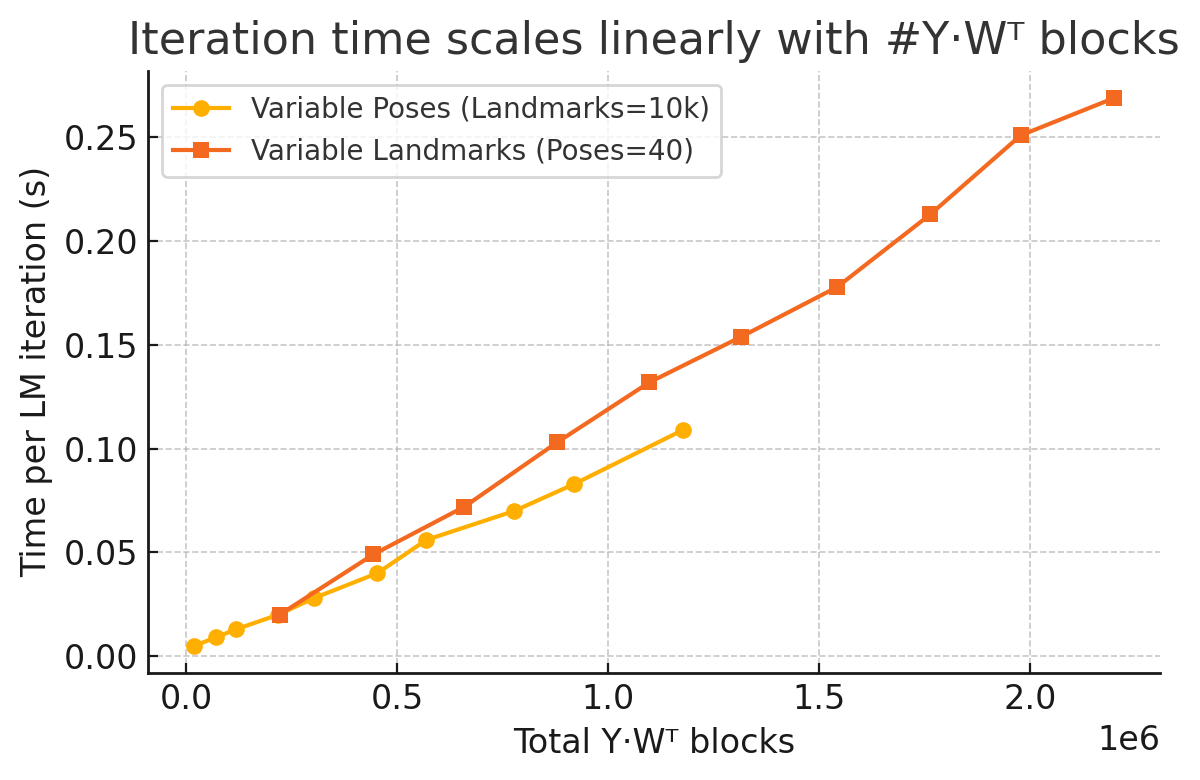
\includegraphics[width=\linewidth]{figs/synth_scaling_YWt}
  \caption{Time per LM iteration on the Core~i9-9900K as a
    function of the number of $\mathbf Y\mathbf W^{\!\top}$ tiles
    in the synthetic scalability suite.  \emph{Circles:} landmarks
    fixed (10 k) while poses increase.  \emph{Squares:} poses fixed
    (40) while landmarks increase. The shared slope
    ($\approx$\SI{0.11}{\micro\second} per tile) indicates that
    $\mathbf{Y}\mathbf{W}^{\!\top}$ multiplication dominates runtime.}
  \label{fig:results_scaling_synth}
\end{figure}

\subsection{Ablation Study}
\label{subsec:results_ablation}
\paragraph{(a) Impact of T\textsuperscript{2}SC.} Table~\ref{tab:ablate_t2sc} shows that disabling 
T$^{2}$SC consistently slows performance on the memory-bandwidth-limited A53 by 2.3–3.2$\times$. 
On the i9, which has a much larger cache, the benefits are even more pronounced on smaller 
problems (up to 12.9$\times$) but diminish as the total tile memory footprint grows. Nonetheless, 
it provided a clear net benefit in all tested scenarios.

\paragraph{(b) Single vs.\ double precision.}  Table~\ref{tab:ablate_precision} confirms that 
float32 reduces memory footprint by 38.9–42.0\% while maintaining $\chi^{2}$ accuracy within 
0.01\% of double‑precision results, with no observable loss in convergence quality.

\begin{table}[h]
\caption{Ablation (a): T$^{2}$SC on/off runtime comparison (ms).}
\label{tab:ablate_t2sc}
\centering
\begin{tabular}{@{}lcccc@{}}
\toprule
& \multicolumn{2}{c}{A53} & \multicolumn{2}{c}{i9} \\
\cmidrule(lr){2-3} \cmidrule(lr){4-5}
Dataset & ON & OFF & ON & OFF \\
\midrule
Ladybug‑1   & 45.6  & 147.3 & 3.9  & 50.4 \\
Dubrovnik‑1 & 184.9 & 315.3 & 22.9 & 96.1 \\
Ladybug‑2   & 82.1  & 238.0 & 6.5  & 78.4 \\
Trafalgar‑3 & 164.2 & 300.1 & 32.5 & 106.0 \\
Ladybug‑3   & 187.8 & 502.0 &  15.3 & 169.0 \\
\bottomrule
\end{tabular}
\end{table}

\begin{table*}[h]
\caption{Ablation (b): float32 vs double precision comparison.}
\label{tab:ablate_precision}
\centering
\begin{tabular}{@{}lccc@{}}
\toprule
Dataset & $\chi^{2}_{\text{f32}}$ & $\chi^{2}_{\text{f64}}$ & RAM \% save \\
\midrule
Ladybug‑1   & 26775.908 & 26783.331 & 38.9\% \\
Dubrovnik‑1 & 36067.785 & 36067.835 & 39.2\% \\
Ladybug‑2   & 34318.758 & 34318.709 & 40.3\% \\
Trafalgar‑3 & 123822.656 & 123820.275 & 39.0\% \\
Ladybug‑3   & 119939.984 & 119940.173 & 42.0\% \\
\bottomrule
\end{tabular}
\end{table*}

\subsection{Peak Memory Consumption}
\label{subsec:results_ram}
Table~\ref{tab:peak_ram} contrasts resident set size across different configurations. 
The T$^{2}$SC pipeline requires 2.1–2.5$\times$ more memory than the baseline version, 
with peak usage reaching \SI{290.4}{MB} on the largest dataset. Interestingly, our baseline 
(T$^{2}$SC off) uses less memory than g2o on most datasets, while the full T$^{2}$SC version 
trades memory for significant speed improvements. Future work will explore tile compression 
and out‑of‑core variants.

\begin{table}[h]
\caption{Peak RAM usage (values in MB).}
\label{tab:peak_ram}
\centering
\begin{tabular}{@{}lccccc@{}}
\toprule
& \multicolumn{5}{c}{Dataset} \\
\cmidrule(lr){2-6}
Implementation & Ladybug-1 & Dubrovnik-1 & Ladybug-2 & Trafalgar-3 & Ladybug-3 \\
\midrule
Ours (+T$^{2}$SC) & 101.7 & 219.2 & 148.5 & 206.0 & 290.4 \\
Ours (-T$^{2}$SC) &  48.0 & 104.2 &  64.6 &  94.9 & 115.8 \\
g2o             &  52.9 &  104.4 &  74.3 &  98.4 & 132.8 \\
\bottomrule
\end{tabular}
\end{table}

\subsection{Discussion and Limitations}
\label{subsec:results_discussion}
The results reveal distinct performance characteristics across platforms. On the i9, the 
large \SI{16}{MB} LLC enables cache‑resident tile processing, delivering 2.3–8.8$\times$ 
speed‑ups over g2o. The effectiveness of T$^{2}$SC varies with problem size; while smaller 
problems see dramatic acceleration (up to 12.9$\times$), the advantage diminishes for larger 
problems as tile memory begins to exceed cache capacity. On the A53 platform, where memory 
bandwidth is the primary bottleneck, T$^{2}$SC provides a consistent and significant 
2.3–3.2$\times$ speed-up. This suggests our contiguous storage and batched BLAS approach is 
highly effective in memory-constrained scenarios. A key limitation is memory overhead: T$^{2}$SC 
requires 2.1–2.5$\times$ more RAM, reaching \SI{290.4}{MB} on the largest dataset—a significant 
constraint for embedded deployment.
\section{Conclusion}
Lorem ipsum dolor sit amet, consectetur adipiscing elit. Donec consectetur
hendrerit turpis, vel sollicitudin mauris hendrerit vel. Phasellus sit amet
lobortis nisi.

Praesent tincidunt sem vel libero fermentum, sed facilisis turpis consectetur.
Fusce sed ligula id arcu venenatis pretium.

% \begin{table}[b]
%   \caption{Future-work milestones (placeholder)}
%   \label{tab:conclusion_future}
%   \centering
%   \begin{tabular}{@{}ll@{}}
%     \toprule
%     Milestone & Target Venue \\ \midrule
%     GPU backend & ICCV 2026 \\
%     FPGA pipeline & ICRA 2027 \\ \bottomrule
%   \end{tabular}
% \end{table}


% ---------- Acknowledgment ----------
\section*{Acknowledgment}
% TODO: Add funding and collaboration acknowledgments
This work was supported by …

% ---------- References ----------
\bibliography{bib/references}

% ---------- Appendix ----------
% \clearpage
% \newpage
\onecolumn
\appendix
% =============================================================================
% APPENDIX
% =============================================================================
\section{Supplementary Material}
\label{app:supplementary}

% TODO: Add supplementary content here
% Examples of what could go in appendices:
% - Detailed derivations
% - Additional experimental results
% - Algorithm pseudocode
% - Hardware specifications
% - Extended performance tables

\subsection{Detailed Algorithm Derivations}
\label{app:derivations}

% TODO: Add mathematical derivations that were too detailed for the main text

\subsection{Additional Experimental Results}
\label{app:additional_results}

% TODO: Add extended experimental results, additional datasets, or 
% performance comparisons that couldn't fit in the main results section

\subsection{Implementation Detailssdsd}
\label{app:implementation}

% --------------------------------------------------------------------
% OptimizerHLS -- Block-Structured BA-LM Solver (Implementation Detail)
% --------------------------------------------------------------------
\begin{algorithm}[H]
\caption{Detailed Block-Structured BA--LM Solver with Scaling and Schur Complement}
\begin{algorithmic}[1]
\small
\Require Scaled tolerance $\varepsilon_{\mathrm{g}}$, damping $\mu$, current pose/landmark parameters $\mathbf{p}_1,\mathbf{p}_2$, observations $\mathbf{x}$, information $\boldsymbol{\Sigma}^{-1}$
\Ensure Increment $\delta\mathbf{p}$
% ------------------ Stage 0: Pre-processing ------------------
\State Compute dense column norms $n_i \gets \lVert \mathbf{J}_{:i} \rVert_2^2$; $s_i \gets 1/\sqrt{n_i+\varepsilon}$
\State Scale Jacobian blocks $\widetilde{\mathbf{J}}_{:i} \gets s_i\,\mathbf{J}_{:i}$ and residual $\widetilde{\boldsymbol{\varepsilon}} \gets \boldsymbol{\Sigma}^{\!-1/2}\,(\mathbf{x}-f(\mathbf{p}))$
% ------------------ Stage 1: Block accumulation ------------------
\ForAll{edge $e=(i,j)$}
  \State $\mathbf{W}_{ij} \mathrel{+}= \widetilde{\mathbf{J}}_{1}(e)^{T}\widetilde{\mathbf{J}}_{2}(e)$
  \State $\mathbf{A}_{i} \mathrel{+}= \widetilde{\mathbf{J}}_{1}(e)^{T}\widetilde{\mathbf{J}}_{1}(e)$;
  $\mathbf{B}_{j} \mathrel{+}= \widetilde{\mathbf{J}}_{2}(e)^{T}\widetilde{\mathbf{J}}_{2}(e)$
  \State $\mathbf{b}_{1,i} \mathrel{+}= \widetilde{\mathbf{J}}_{1}(e)^{T}\widetilde{\boldsymbol{\varepsilon}}(e)$;
  $\mathbf{b}_{2,j} \mathrel{+}= \widetilde{\mathbf{J}}_{2}(e)^{T}\widetilde{\boldsymbol{\varepsilon}}(e)$
\EndFor
% ------------------ Stage 2: LM damping ------------------
\ForAll{$i$} $\mathbf{A}_{i} \gets \mathbf{A}_{i}+\mu\mathbf{I}$ \EndFor;
\ForAll{$j$} $\mathbf{B}_{j} \gets \mathbf{B}_{j}+\mu\mathbf{I}$ \EndFor
% ------------------ Stage 3: Landmark elimination ------------------
\ForAll{$j$} $\mathbf{B}^{-1}_{j} \gets \text{LDLT}(\mathbf{B}_j)$ (SVD fallback) \EndFor
\ForAll{$(i,j)$} $\mathbf{Y}_{ij} \gets \mathbf{W}_{ij}\mathbf{B}^{-1}_{j}$ \EndFor
% ------------------ Stage 4: Reduced Hessian & Gradient ------------------
\For{$i=1$ \textbf{to} $m$}
  \State $\mathbf{H}_{ii} \gets \mathbf{A}_{i}$
  \State $\mathbf{b}_{\mathrm{act},i} \gets \mathbf{b}_{1,i}$
\EndFor
\ForAll{pose pair $(i,k)$ sharing landmarks}
  \State $\mathbf{H}_{ik} \gets \mathbf{0}$
\EndFor
\ForAll{edge $e=(i,j)$}
  \State $\mathbf{H}_{ii} \mathrel{-}= \mathbf{Y}_{ij}\mathbf{W}_{ij}^T$
  \State $\mathbf{b}_{\mathrm{act},i} \mathrel{-}= \mathbf{Y}_{ij}\mathbf{b}_{2,j}$
  \ForAll{pose $k\,(k<i)$ observing $j$}
    \State $\mathbf{H}_{ik} \mathrel{-}= \mathbf{Y}_{ij}\mathbf{W}_{kj}^T$
  \EndFor
\EndFor
% ------------------ Stage 5: Solve for pose increments ------------------
\State Solve $\mathbf{H}\,\delta\mathbf{p}_1 = \mathbf{b}_{\mathrm{act}}$ (LDLT, fallback LU)
% ------------------ Stage 6: Back-substitution for landmarks ------------------
\For{$j=1$ \textbf{to} $n$}
  \State $\delta\mathbf{p}_{2,j} \gets \mathbf{B}^{-1}_{j}\Bigl(\mathbf{b}_{2,j}-\sum_{i}\mathbf{W}_{ij}^{T}\,\delta\mathbf{p}_{1,i}\Bigr)$
\EndFor
% ------------------ Stage 7: Un-scaling ------------------
\State $\delta\mathbf{p} \gets \delta\mathbf{p} \oslash \mathbf{s}$ %\Comment{Element-wise unscale}
\State \Return $\delta\mathbf{p}$
\end{algorithmic}
\end{algorithm}

\paragraph{Design Highlights.}
\begin{itemize}[leftmargin=*]
  \item \textbf{Block-Diagonal Storage:} Pose ($\mathbf{A}_i$) and landmark ($\mathbf{B}_j$) blocks are kept in contiguous column-major slabs to maximise BLAS level-3 throughput.
  \item \textbf{Edge-Centric Accumulation:} The edge lists \verb|v1_edge|, \verb|v2_edge| drive accumulation loops without expensive indirections.
  \item \textbf{Pose-Pair Hashing:} Off-diagonal look-ups use the compact index $k=\tfrac{i(i-1)}{2}+j$ into \verb|v1_edge_pairs| to achieve $O(1)$ co-observation access.
  \item \textbf{Mixed Precision:} Jacobians are differentiated in \texttt{double} yet stored as the compile-time \texttt{Scalar} type (\texttt{float} by default).
  \item \textbf{Jacobi Scaling:} Column-wise norms yield scale vector $\mathbf{s}$; its inverse rescales Jacobian columns in place, improving condition numbers.
  \item \textbf{Pipeline Mode:} When \texttt{usePipeline} is enabled, W-block assembly runs asynchronously while the CPU assembles Schur tiles, hiding memory latency.
\end{itemize}
% -------------------------------------------------------------------- 

\end{document}
